\documentclass[document.tex]{subfiles}
\begin{document}
\section*{Exercise 1:}

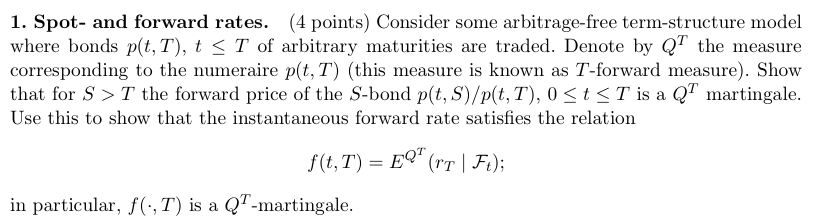
\includegraphics[width=\textwidth]{ex1.png}

From the fundamental theorem of calculus we get following relationship between $f(t,\cdot)$ and $p(t, )$ \\
\begin{align*}
	p(t,T) = \exp \lb - \int^T_t f (t,u) du \rb \text{see lecture notes (8.1)}
\end{align*}
This implies 
\begin{align*}
	f(t,T) = - \frac{\partial \ln p (t,T) }{\partial T}
\end{align*}
since the instantaneous short-rate of interest is $r(t) = f(t,t)$\\
to show that $f(t,T) = \E^{Q^T} \lb f(T,T) \rb $ it is sufficient to show
\begin{align*}
	- \frac{\partial \ln p (t,T) }{\partial T} = \E^{Q^T} \lb r(T) \rb 
\end{align*}
the price process of the zero coupon dicounted with the money market acount $B_t = \exp(\int_0^t r_s ds)$
under the bond price measure is a martingale
\begin{align*}
	\frac{p(t,T)}{B_t} = \E^{Q^B} \lb  \frac{p\lb T,T\rb}{B_T} \rb
\end{align*}
since the price of a zero coupn bond at maturity is 1. We can rewrite this as follows 
\begin{align*}
	p(t,T) = \E^{Q^B} \lb  \frac{B_t}{B_T} \rb = \E^{Q^B} \lb  \exp \lb - \int_t^T r(s) ds \rb \rb 
\end{align*}
Taking the derivative with respect to $T$ gives us	
\begin{align*}
	- \frac{\partial p (t,T) }{\partial T} = \E^{Q^B} \lb  \exp \lb - \int_t^T r(s) ds \rb r(T) \rb   
\end{align*}
Now we just have to change measure from the money account meassure $Q^B$ to the T-forward measure $Q^T$  
with the Radon Nikodyn derivative  $\frac{d Q^B}{dQ^T} = \frac{p\lb t,T \rb}{\exp \lb - \int_t^T r(s) ds \rb }$
\begin{align*}
	- \frac{\partial p(t,T)}{\partial T} = \E^{Q^T} \lb  \exp \lb - \int_t^T r(s) ds \rb r(T)  
	\frac{p\lb t,T \rb}{\exp \lb - \int_t^T r(s) ds \rb } \rb 
	  = p \lb t,T \rb  \E^{Q^T} \lb r(T)  \rb 
\end{align*}
Since in general $\frac{d}{dx} \ln g(x) = \frac{g'(x)}{g(x)}$
we end up with the wanted result 
\begin{align*}
	- \frac{\partial \ln p (t,T) }{\partial T} = \E^{Q^T} \lb r(T) \rb 
\end{align*}

\end{document}
